\section{Receiver Position From Code Observations}
	The receiver position problem in GPS is as follows: $m\geq4$ satellites are tracked. We assume that at any time we can compute their coordinates. All distances between the satellites and the unknown receiver position (X,Y,Z) are observed. The receiver clock is imprecise so we also have to estimate its offset dt compared to GPST.
	
	There are four unknowns X,Y,Z, dt so we must track at least four satellites in order to obtain a position. Most often we track m = 8 to 10 satellites.
	
	The GPS literature mentions several methods for solving the problem. The ordinary least-squares method is a natural choice. There are suggestions on weighting the observations to satellites close to the enith more heavily than observations to satellites closer to the horizon, see e.g. Euler $\&$ Goad (1991). In the 1990s Clyde Goad suggested to search over all possible positions to find the one with the smallest sum of squares of errors. In 1985 Bancroft outlined a method based on inner products, which assumes m = 4. Kleusberg in 1994 describes a method which eliminates dt and squares the observation equations, again for m = 4. Such an assumption is not relevant today with so many satellites.
	
	Consider a GPS signal traveling from satellite k to receiver i = 1, always k = 1,..., m.The signal is transmitted at time $t^k$ measured by the satellite clock. It arrives at time $t^i$ measured by the receiver clock. The travel time is $\tau^k_i$. If c is the velocity of light, then the pseudorange $P^k_i$ is defined by
	\begin{equation}\label{eq:9.13}
		t_i-t^k=\tau^k_i=P^k_i/c \quad or\quad  t^k=t_i-P^k_i/c 
	\end{equation}
	
	Clocks do not behave perfectly, so we define clock offsets dt :
	
	Receiver clock offset $dt_i$:
	\begin{equation}\label{9.14}
		t_i = t^{GPST}+dt_i
	\end{equation} 
	Satellite clock offset $dt^k$:
	\begin{equation}\label{eq:9.15}
		t^k = (t-\tau ^k_i)^{GPST}+dt^k
	\end{equation}
	The satellite clock correction is defined using $a_0$,$a_1$,$a_2$ from the ephemeris:
	\begin{equation}\label{eq:9.16}
		dt^k=a_0+a_1(t^k-t_{oe})+a_2(t^k-t_{oe})^2+\ldots
	\end{equation}
	
	After applying dtk , the satellite clock is known to within $\pm 10$ ns and always $|dt_i|<1$ms.
	
	A measurement epoch $t_i$ is defined in terms of the receiver clock. This epoch is common to all signals received from the tracked satellites. However, the signals were between transmitted receiver at $(t-\tau ^k_i)^{GPST}$which obviously depends on $\mu ^k_i$. or in other words the range between receiver i and satellite k.so a first task is to compute transmit time $t^k$at satellite the range k. This involves \ref{eq:9.15} and \ref{eq:9.16}.
	\begin{figure}
	\centering
	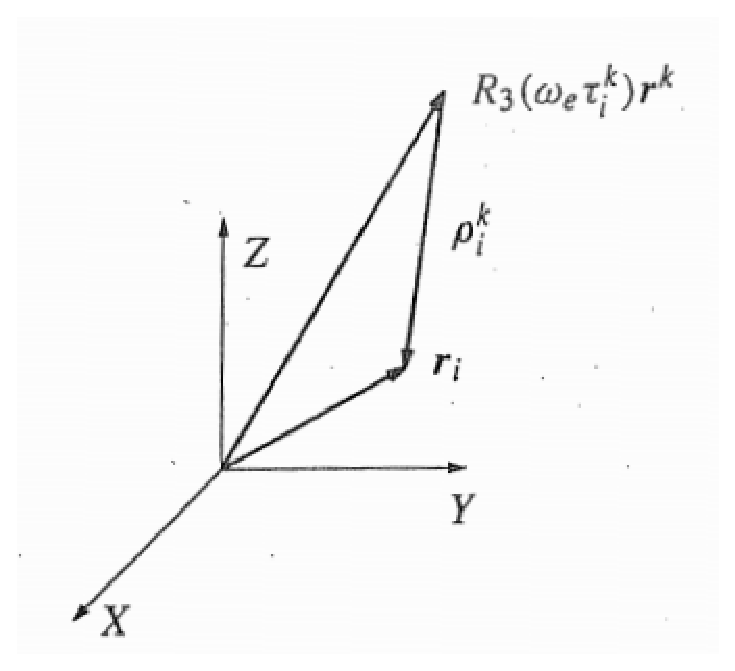
\includegraphics[width=0.7\linewidth]{TeX_files/Part03/chapter09/image/9-12}
	\caption{Receiver position $r_i$ in an Earth Centered Inertial coordinate system and satellite position $R_3(\omega_e \tau ^k_i)r^k$ in an Earth Centered and Earth Fixed coordinate system. The first position is transformed into the ECEF system by a rotation around the Z-axis by the angle $\omega_e \tau ^k_i$}
	\label{fig:9-12}
	\end{figure}

	According to the ephemerides all satellite positions are calculated in WGS84 which is an Earth Centered and Earth Fixed (ECEF) system. This implies that we must rotate the satellite position vector about the 3-axis an amount equal to the angular rotation of the Earth in the time it takes the signal to travel from the satellite to the receiver. The height of a GPS satellite is about 20000 km. Thus the signal transit time is about 66 ms. The Earth rotates 15 arcsec per second so the angular displacement of the Earth about its rotation axis during signal travel is roughly 1 arcsec. So if ECEF coordinates are used and the correction is not applied, the recovered station coordinates will be biased by about one arcsec in longitude.
	
	According to Figure \ref{fig:9-12} the distance between satellite k and receiver i——corrected for Earth rotation——is defined by
	\begin{equation}\label{eq:9.17}
		\rho ^k_i = \Arrowvert R_3(\omega_e\tau^k_i)r^k(t-\tau^k_i)_{inert}-r_i(t)_{ECEF} \Arrowvert = 
		\Arrowvert \begin{bmatrix}
		X^k \\ Y^k \\ Z^k
		\end{bmatrix}-
		\begin{bmatrix}
		X_i \\ Y_i \\ Z_i
		\end{bmatrix} \Arrowvert
	\end{equation}
	
	The matrix R3 accounts for rotation by the angle $\omega_e \tau^k_i$ while the signal is traveling:
	\begin{equation}
	R_3(\omega_e\tau^k_i) =
		\begin{bmatrix}
			 \cos(\omega_e\tau^k_i) & \sin(\omega_e\tau^k_i) & 0 \\
			-\sin(\omega_e\tau^k_i) & \cos(\omega_e\tau^k_i) & 0 \\
			0 & 0 & 1
		\end{bmatrix}
	\end{equation}
	
	The travel time from (the signal generator in) the satellite k to (the signal correlator in) the receiver i is denoted $\tau$. The rotation rate of the Earth is $\omega_e$. Position vectors in the ECEF system are denoted $r(t)_{ECEF}$. The argument t emphasizes dependence on time.
	
	The basic equation for a pseudorange observation looks like
	\begin{equation}\label{eq:9.19}
		P^k_i(t) = \rho^k_i+I^k_i+T^k_i-c(dt^k(t-\tau^k_i)-dt_i(t))-e^k_i
	\end{equation}
	
	The ionospheric delay is $I^k_i$ , the tropospheric delay is $T^k_i$ , and c denotes the vacuum speed of light; and $e^k_i$ denotes an error.
	\begin{figure}
		\centering
		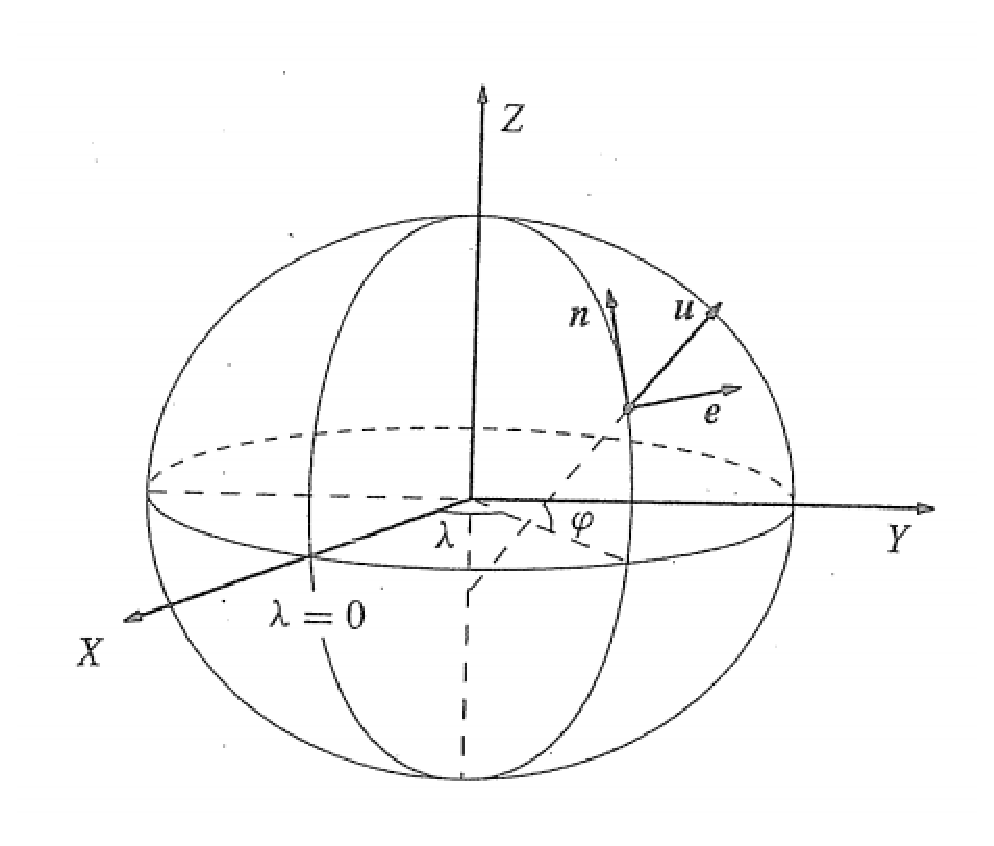
\includegraphics[width=0.7\linewidth]{TeX_files/Part03/chapter09/image/9-13}
		\caption{Topocentric coordinate frame(e,n,u)}
		\label{fig:9-13}
	\end{figure}

	So we need to transform a topocentric vector x: into a local e,n,u coordinate system,with u in the direction of the plumb line, n pointing north, and e pointing east, as shown in Figure \ref{fig:9-13}. The topocenter is given by the geocentric vector X, and the three unit vectors go into the orthogonal matrix F which was already introducedin (3.31):
	\begin{equation}\label{eq:9.20}
		F = \begin{bmatrix}
		e & n & u
		\end{bmatrix}=
		\begin{bmatrix}
		-\sin \lambda & -\sin\varphi\cos\lambda & \cos\varphi\cos\lambda \\
		 \cos \lambda & -\sin\varphi\sin\lambda & \cos\varphi\sin\lambda \\
		 0 & \cos\varphi & \sin\varphi
		\end{bmatrix}
	\end{equation}
	
	Knowing preliminary values of the Cartesian coordinates $(X^0_i,Y^0_i,Z^0_i)$ we can compute the geographical coordinates $(\varphi,\lambda)$ for the receiver and hence the entries of the matrix F.Now $(E,N,U)=F^Tx$. Immediately we have azimuth, elevation angle, and length:
	\begin{table}
		\begin{tabular}{ll}
			Azimuth: 		 & $Az = \arctan(E/N)$ \\ 
			Elevation angle: & $El=\arctan(U/\sqrt{N^2+E^2})$ \\ 
			Length:			 & $s=\Arrowvert x \Arrowvert$ \\ 
		\end{tabular} 
	\end{table}
	
	Knowing the elevation angle we can compute $T^k_i$. The ionospheric delay $I^k_i$ is set to zero as we do not know better, and $dt^k$ was computed from \ref{eq:9.16}. The unknowns are $dt_i$ and the three coordinates$(X_i,Y_i,Z_i)$ which are hidden in $\rho^k_i$. So we start by linearizing \ref{eq:9.19}:
	\begin{equation}\label{eq:9.21}
		-\dfrac{X^k-X^0_i}{(\rho^k_i)^0}x_i-\dfrac{Y^k-Y^0_i}{(\rho^k_i)^0}y_i-\dfrac{Z^k-Z^0_i}{(\rho^k_i)^0}z_i+1(c\,dt_i)=(P^k_i)_{obs}-(P^k_i)^0-e^k_i=b_i-e^k_i
	\end{equation}
		
	In a first approximation we put $\rho^k_i\approx(\rho^k_i)^0=(P^k_i)^0$,which is the geometric distance as calculated from the preliminary coordinates of satellite and receiver.The number $b_i$ denotes the observed minus the calculated value.
	
	The preliminary value of $(P^k_i)^0$ may be the origin or computed from the possible preliminary coordinates $(X^0_i,Y^0_i,Z^0_i)$ of the receiver. It is corrected for receiver clock offset $dt_i$ , with first guess $dt_i=0$.If the preliminary values are good the right side $b_i$ is small. Note that the direction cosines use the components described by \ref{eq:9.17}.
	
	The linearized observation equations are of the type described by \ref{eq:9.21} and we arrange the unknowns as $x=(x_i,y_i,z_i,c\,dt_i)$:
	\begin{equation}\label{eq:9.22}
		Ax=\begin{bmatrix}
		-\dfrac{X^1-X_i}{\rho^1_i} & -\dfrac{Y^1-Y_i}{\rho^1_i} & -\dfrac{Z^1-Z_i}{\rho^1_i} & 1 \\
		-\dfrac{X^2-X_i}{\rho^2_i} & -\dfrac{Y^2-Y_i}{\rho^2_i} & -\dfrac{Z^2-Z_i}{\rho^2_i} & 1 \\
		\vdots & & & \\
		-\dfrac{X^3-X_i}{\rho^3_i} & -\dfrac{Y^3-Y_i}{\rho^3_i} & -\dfrac{Z^3-Z_i}{\rho^3_i} & 1 \\
		\end{bmatrix}
	\end{equation}
	
	Note that the factors c and $dt_i$ stay together in one product. This is done for numerical reasons. The unknown $c\,dt_i$ has the same dimension as the other unknowns, namely length.However some people like to estimate the term as time. This can be done by using the unknown $dt_i$ together with a reasonably small coefficient like $c x 10^9$ yielding $dt_i$ in ns.
	
	Row-wise the first three columns of A contain the direction cosines for the vector between satellite and receiver. The least-squares solution is
	\begin{equation}\label{eq:9.23}
		\begin{bmatrix}
			\hat{x}_i \\ \hat{y}_i \\ \hat{z}_i \\ \hat{c\,dt_i}
		\end{bmatrix}
		=(A^T\Sigma^{-1}A)^{-1}A^T\Sigma^{-1}b
	\end{equation}
	
	The pseudorange observations are considered independent with equal variance so $e\sim N(0,\sigma^2I)$. In other words the vector e has zero mean and covariance matrix $\Sigma = \sigma^2I$. If this assumption is correct, \ref{eq:9.23}is simplified to
	\begin{equation}\label{eq:9.24}
		\begin{bmatrix}
			\hat{x}_i \\ \hat{y}_i \\ \hat{z}_i \\ \hat{c\,dt_i}
		\end{bmatrix}
		=(A^TA)^{-1}A^Tb
	\end{equation}
	The iterated receiver coordinates are
	\begin{equation}\label{eq:9.25}
		\hat{X}_i=X^0_i+\hat{x}_i,\quad \hat{Y}_i=Y^0_i+\hat{y}_i,\quad and \quad \hat{Z}_i=Z^0_i+\hat{z}_i,
	\end{equation}
	The iteration involving \ref{eq:9.22},\ref{eq:9.24} and \ref{eq:9.25} is repeated until the norm $\Arrowvert x\Arrowvert=\sqrt{x^Tx}$ is smaller than $10^2$, say
	
	We conclude by establishing a data set consisting of one epoch. It contains PRN`s k = 1,4,7,13,20,24,25 as in Table\ref{tab:9.4}. The pseudoranges are corrected according to the following equation:
	\begin{equation}\label{eq:9.26}
		P = observed pseudorange + c\,dt^k-T.
	\end{equation}
	
	The M-file easy3 calls satpos which computes the positions at transmission time.
	\begin{table}
		\caption{Coordinates $(X^k,Y^k,Z^k)$ of satellites present in a certain epoch. The observed pseudoranges are denoted $P^k$}
		\label{tab:9.4}
		\begin{tabular}{crrrr}
			\hline
			PRN & 1 & 4 & 7 & 13 \\ 
			\hline
			$X^k[m]$ & 14789533.14 &  11784778.93 &  20131229.62 & 22053478.89  \\ 
			$Y^k[m]$ &  7334543.20 & -10589833.27 & -17092167.32 & -4245955.78  \\ 
			$Z^k[m]$ & 20976503.11 &  21427005.76 &   1367264.01 & 14103264.45  \\ 
			$P^k[m]$ & 20589966.21 &  21428477.36 &  24767161.79 & 21266276.50  \\ 
			\hline
		\end{tabular} 
		\begin{tabular}{crrr}
			\hline
			PRN & 20 & 24 & 25 \\
			\hline
			$X^k[m]$ & 12654506.52 &  -1514708.63 & -9091147.00 \\
			$Y^k[m]$ & 17685295.10 & -16394944.97 & 13349830.35 \\ 
			$Z^k[m]$ & 15150460.02 &  21142855.83 & 21347346.61 \\ 
			$P^k[m]$ & 21871195.29 &  23851770.76 & 24109819.35 \\ 
			\hline
		\end{tabular}
	\end{table}	
		
	Knowing the satellite positions and the measured pseudoranges we estimate the receiver coordinates and receiver clock offset $\hat{c\,dt}$ by least squares:
		
	The receiver clock offset compared to GPS time is $\hat{dt} = 0.377 ms$. The result is obtained after 6 iterations. The standard deviation of the receiver position is 2.3 m, see Chapter 4.
	\subsection{easy3}\label{subsec:easy3}
		In easy3 we compute a receiver’s ECEF position from RINEX o- and n-files. Only pseudo-ranges are used. Transmit time in GPST is $(t_i-\tau^k_i)^{GPST}$ which is used for computation of the satellite position.
		
		Next we quote a central piece of code that is applied in any positional computation.It may be difficult to grasp at the very first reading, but we try to put words to it: The goal is to find the epoch in GPST at which a particular signal was transmitted from a given satellite. We know the epoch $t_i$, counted by the receiver clock, when some observations were taken. The signal was transmitted P / c seconds earlier from the satellite. We know the pseudorange P and the velocity of light c. Next we compute the satellite clock offset tcorr from the parameters $a_0$ and $a_1$ given in the ephemerides. However, this quantity depends on the time elapsed since the ephemeris was issued at tOc. So the tcorr value can only be obtained through an iteration, so you see tcorr appears twice on the left side. Knowing tcorr we finally can compute the true GPST when the signal was transmitted and finally the satellite position at that moment. The code is as follows:
		\begin{lstlisting}
			k = col_Eph(i);
			tx_RAW = time - obs(i)/v_light;
			tOc = Eph(21,k);
			dt = check_t(tx_RAW-tOc);
			tcorr = (Eph(2,k) * dt + Eph(20,k)) * dt + Eph(19,k);
			tx_GPS = tx_RAW- tcorr;
			dt - check_t(tx_GPS-tOc);
			tcorr = (Eph(2,k) * dt -f Eph(20,k)) * dt + Eph(19,k);
			tx_GPS = tx_RAW-tcorr;
			X = satpos(tx_GPS, Eph(:,k));			
		\end{lstlisting}
		The following code corrects for the Earth rotation while the signal travels from satellite to receiver. As described in (9.18) the satellite position must be rotated around the Z-axis by the angle $\omega_e\tau^k_i$. In the first iteration we do not know the exact travel time and set it to 0.072 s. The tropospheric delay is set to 0 s. In the next iteration we estimate the elevation angle for the satellite, as this angle el is important for computing the tropospheric delay.It is implemented as tropo.
		\begin{lstlisting}
			if iter == 1
				traveltime = 0.072;
				Rot_X = X;
				trop = 0;
			else
				rho2 - (X(1)-pos(1))~ 2 + (X(2)-pos(2))~ 2 + (X(3)-pos(3))~ 2;
				traveltime = sqrt(rho2)/v_light;
				Rot_X = e_i'_corr(traveltime,X);
				rho2 = (Rot_X(l)-pos(1)) ^2 + (Rot_X(2)-pos(2))"2 -r (Rot_X(3)-pos(3)) ^2;
				[az,el,dist] = topocent(pos(1:3 /:),Rot_X-pos(1:3,:));
				if iter == nojterations, El(i) = el; end
				trop = tropo(sin(el * dtr), 0.0, 1013.0, 293.0, 50.0, 0.0, 0.0, 0.0);
			end
		\end{lstlisting}
		The key code for the receiver position computation is a separate M-file called $recpo_ls$.
		
		We open a RINEX o-file and read all the pseudoranges given at an epoch. With given satellite positions from easy2, we compute the receiver position.
		
		The computationis repeated over 20 epochs. Each positionis theresult of an iterative least-squares procedure. The variation of the position relative to the first epoch is shown in Figure \ref{fig:9-14}. The variationin coordinate values is typically less than 5 m.
		\begin{figure}[h]
			\centering
			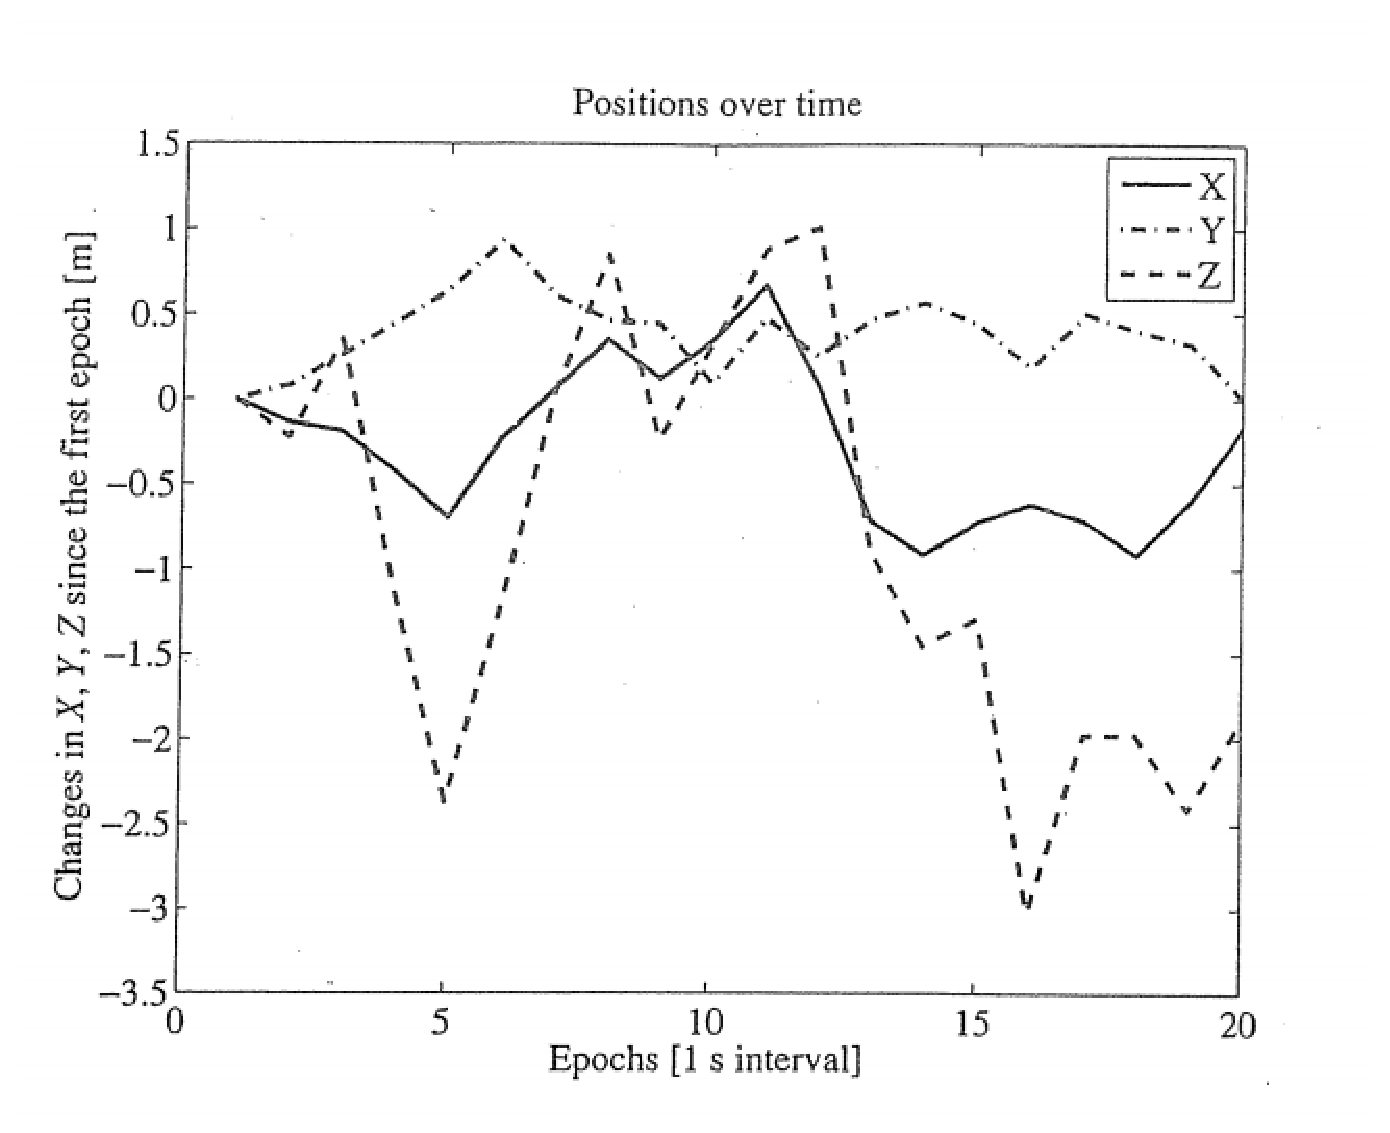
\includegraphics[width=0.7\linewidth]{TeX_files/Part03/chapter09/image/9-14}
			\caption{Receiver postion from pseudoranges over time:X,Y,Z coordinates}
			\label{fig:9-14}
		\end{figure}
		
